\documentclass[a5paper,headsepline,titlepage,11pt,nnormalheadings,DIVcalc]{scrbook}
\usepackage[a5paper,backref]{hyperref}
\usepackage[papersize={148.5mm,215mm},twoside,bindingoffset=0.5cm,hmargin={2cm,2cm},
				vmargin={2cm,2cm},footskip=1.1cm,driver=dvipdfm]{geometry}
%\usepackage{palatino}
\usepackage{graphicx}
\usepackage{wrapfig}
\usepackage[bahasa]{babel}
\usepackage{fancyhdr}
\usepackage{longtable}
\usepackage{hhline,multirow}
\usepackage{pst-node}

%\setlength{\voffset}{0.5in}
%\setlength{\oddsidemargin}{28pt}
%\setlength{\evensidemargin}{0pt}
\renewcommand{\footrulewidth}{0.5pt}
\lhead[\fancyplain{}{\thepage}]%
      {\fancyplain{}{~}}
\rhead[\fancyplain{}{~}]%
      {\fancyplain{}{\thepage}}
\pagestyle{fancy}
\lfoot[\emph{Ibadat Paskah}]{}
\rfoot[]{\emph{Lingkungan St Petrus Maguwo}}
\cfoot{}

\newcommand{\BU}[1]{\begin{itemize} \item[U:] #1 \end{itemize}}
\newcommand{\BI}[1]{\begin{itemize} \item[I:] #1 \end{itemize}}
\newcommand{\BP}[1]{\begin{itemize} \item[P:] #1 \end{itemize}}
\newcommand{\BPP}[1]{\begin{itemize} \item[Bpk:] #1 \end{itemize}}
\newcommand{\BPW}[1]{\begin{itemize} \item[Ibu:] #1 \end{itemize}}
\newcommand{\namaalm}{Ibu MG Ari Tri Wuryanti~}
\newcommand{\namaromo}{~}
\title{Ibadat/Doa untuk Arwah}
\author{}
\date{2010}
\hyphenation{sa-u-da-ra-ku}
\hyphenation{ke-ri-ngat}
\hyphenation{je-ri-tan}
\hyphenation{hu-bung-an}
\hyphenation{me-nya-dari}
\hyphenation{Eng-kau}
\hyphenation{ke-sa-lah-an}
\hyphenation{ba-gai-ma-na}
\hyphenation{Tu-han}
\hyphenation{di-per-ca-ya-kan}
\hyphenation{men-ja-uh-kan}
\hyphenation{bu-kan-lah}
\hyphenation{per-sa-tu-kan-lah}
\hyphenation{ma-khluk}
\hyphenation{Sem-buh-kan-lah}
\hyphenation{ja-lan}
\hyphenation{mem-bu-tuh-kan}
\hyphenation{be-ri-kan-lah}
\hyphenation{me-ra-sa-kan}
\hyphenation{te-man-ilah}
\hyphenation{mem-bi-ngung-kan}
\hyphenation{di-ka-gum-i}
\hyphenation{ta-ngis-an-Mu}
\hyphenation{mi-lik-ilah}

\renewcommand*\thesection{\arabic{section}.}
\setlength{\parindent}{0mm} 

\begin{document}
\thispagestyle{empty}
%\maketitle
%\newsavebox\IBox
%\sbox\IBox{\includegraphics[scale=0.4]{Saint-Peter-Apostle-e.eps}}

\psset{unit=1in}
\begin{pspicture}(4in,6.0in)
% set up the fonts we use
\DeclareFixedFont{\PT}{T1}{ppl}{b}{it}{0.4in}
\DeclareFixedFont{\PTsmall}{T1}{ppl}{b}{it}{0.3in}
\DeclareFixedFont{\PTsmallest}{T1}{ppl}{b}{it}{0.2in}
\DeclareFixedFont{\PTtext}{T1}{ppl}{b}{it}{11pt}
\DeclareFixedFont{\Logo}{T1}{pbk}{m}{n}{0.2in}
% place the front cover picture
%\rput[cb](2.3,2.5){\usebox\IBox}
% put the text on the front cover
\rput[cb](2.5,5.3){\PTsmall {Ibadat Paskah}}
\rput[cb](2.5,4.8){\PTsmall {Lingkungan St Petrus}}
\rput[cb](2.5,1.1){\PTsmall {11 April 2010}}
\rput[cb](2.5,0.6){\PTsmallest {Wilayah Yohanes de Britto}}
\rput[cb](2.5,0.3){\PTsmallest {Stasi Maguwo}}
\rput[cb](2.5,0.0){\PTsmallest {Paroki Marganingsih Kalasan }}

%\rput[cb](3,-1){\PTsmallest {\namagereja}} 

\end{pspicture}
%\tableofcontents 
\newpage
\thispagestyle{empty}
{~}
\newpage
\setlength{\parskip}{2mm}

\section*{RITUS PEMBUKA}
\subsection*{LAGU PEMBUKA}

\subsection*{SALAM PEMBUKAAN}
\BP{Atas nama Bapa Putera dan Roh Kudus} 
\BU{Amin}
\BP{Semoga damai sejahtera Tuhan kita Yesus Kristus, cinta kasih Allah Bapa dan persekutuan Roh Kudus, selalu beserta kita.}
\BU{Sekarang dan selama-lamanya}

\subsection*{PENGANTAR}
\BP{Bapak Ibu Saudara Saudari Anak-anak yang terkasih dalam Kristus, malam ini kita berkumpul untuk melanjutkan gaung Paskah tahun ini, yang mengambil tema 'Bersyukur dengan bertobat dan berbagi berkat'. Tema yang indah memang. Oleh karena itu pengurus lingkungan St Petrus ingin lebih mengaktualisasikan tema itu dalam kehidupan umat sehari-hari. Setelah ibadat ini, akan dilanjutkan dengan ikrar yang diharapkan lebih membulatkan tekad kita untuk bersyukur, bertobat, dan berbagi berkat.}

\emph{Hening sejenak \dots}
  
\subsection*{PERNYATAAN TOBAT}
\BP{Saudara-saudari yang seiman dalam Kristus, marilah kita membuat diri pantas berada di depan Allah, bersih dari dosa dan kesalahan yang lalu, dengan bertobat dan mohon ampun kepada Allah kita.}

\BP{Saya mengaku \dots}

\BP{Semoga Allah yang mahakuasa mengasihani kita, 
mengampuni dosa kita dan mengantar kita ke dalam hidup 
yang kekal.}

\BU{Amin}

\subsection*{Doa Pembuka} 
\BP{Marilah Berdoa 

Allah yang mahabaik, kami mengucap syukur kepada-Mu karena Engkau senantiasa mendengar dan memperhatikan kami dalam suka dan duka serta selalu menyertai kami dalam perjalanan hidup kami. Kami mohon, semoga iman kami kepadaMu tetap teguh sehingga dapat mengabdi kepadaMu dengan gembira dan penuh rasa syukur. Demi Yesus Kristus, PutraMu, Tuhan dan Pengantara kami, yang hidup dan berkuasa bersama Dikai dan Roh Kudus, kini dan sepanjang masa.
 }

\BU{Amin} 
 
\section*{IBADAT SABDA}
\BP{Saudara-saudari terkasih marilah kita mempersiapkan hati 
dan budi untuk mendengarkan sabda Tuhan.} 

\subsection*{BACAAN PERTAMA}

\BP{Pembacaan dari Surat Rasul Paulus kepada Umat di Kolose (3: 1-17) 

Saudara-saudara, karena itu, kalau kamu dibangkitkan bersama dengan Kristus, carilah perkara yang di atas, di mana Kristus ada, duduk di sebelah kanan Allah.
Pikirkanlah perkara yang di atas, bukan yang di bumi.
Sebab kamu telah mati dan hidupmu tersembunyi bersama dengan Kristus di dalam Allah.

Apabila Kristus, yang adalah hidup kita, menyatakan diri kelak, kamupun akan menyatakan diri bersama dengan Dia dalam kemuliaan.
Karena itu matikanlah dalam dirimu segala sesuatu yang duniawi, yaitu percabulan, kenajisan, hawa nafsu, nafsu jahat dan juga keserakahan, yang sama dengan penyembahan berhala,
semuanya itu mendatangkan murka Allah (atas orang-orang durhaka).

Dahulu kamu juga melakukan hal-hal itu ketika kamu hidup di dalamnya.
Tetapi sekarang, buanglah semuanya ini, yaitu marah, geram, kejahatan, fitnah dan kata-kata kotor yang keluar dari mulutmu.
Jangan lagi kamu saling mendustai, karena kamu telah menanggalkan manusia lama serta kelakuannya,
dan telah mengenakan manusia baru yang terus-menerus diperbaharui untuk memperoleh pengetahuan yang benar menurut gambar Khaliknya;
dalam hal ini tiada lagi orang Yunani atau orang Yahudi, orang bersunat atau orang tak bersunat, orang Barbar atau orang Skit, budak atau orang merdeka, tetapi Kristus adalah semua dan di dalam segala sesuatu.

Karena itu, sebagai orang-orang pilihan Allah yang dikuduskan dan dikasihi-Nya, kenakanlah belas kasihan, kemurahan, kerendahan hati, kelemahlembutan dan kesabaran.
Sabarlah kamu seorang terhadap yang lain, dan ampunilah seorang akan yang lain apabila yang seorang menaruh dendam terhadap yang lain, sama seperti Tuhan telah mengampuni kamu, kamu perbuat jugalah demikian.
Dan di atas semuanya itu: kenakanlah kasih, sebagai pengikat yang mempersatukan dan menyempurnakan.

Hendaklah damai sejahtera Kristus memerintah dalam hatimu, karena untuk itulah kamu telah dipanggil menjadi satu tubuh. Dan bersyukurlah.
Hendaklah perkataan Kristus diam dengan segala kekayaannya di antara kamu, sehingga kamu dengan segala hikmat mengajar dan menegur seorang akan yang lain dan sambil menyanyikan mazmur, dan puji-pujian dan nyanyian rohani, kamu mengucap syukur kepada Allah di dalam hatimu.
Dan segala sesuatu yang kamu lakukan dengan perkataan atau perbuatan, lakukanlah semuanya itu dalam nama Tuhan Yesus, sambil mengucap syukur oleh Dia kepada Allah, Bapa kita.

Demikianlah sabda Tuhan }

\BU{Syukur kepada Allah} 

\subsection*{Antar Bacaan} 

\subsection*{Bacaan Injil} 

\BP{Tuhan sertamu} 
\BU{Dan sertamu juga} 
\BP{Inilah Injil Yesus Kristus menurut Matius (11:25-30)} 
\BU{Dimuliakanlah Tuhan}

\BP{Pada waktu itu berkatalah Yesus: "Aku bersyukur kepada-Mu, Bapa, Tuhan langit dan bumi, karena semuanya itu Engkau sembunyikan bagi orang bijak dan orang pandai, tetapi Engkau nyatakan kepada orang kecil.

Ya Bapa, itulah yang berkenan kepada-Mu.

Semua telah diserahkan kepada-Ku oleh Bapa-Ku dan tidak seorangpun mengenal Anak selain Bapa, dan tidak seorangpun mengenal Bapa selain Anak dan orang yang kepadanya Anak itu berkenan menyatakannya.

Marilah kepada-Ku, semua yang letih lesu dan berbeban berat, Aku akan memberi kelegaan kepadamu.

Pikullah kuk yang Kupasang dan belajarlah pada-Ku, karena Aku lemah lembut dan rendah hati dan jiwamu akan mendapat ketenangan.

Sebab kuk yang Kupasang itu enak dan beban-Kupun ringan."

Demikianlah Injil Tuhan} 

\BU{Terpujilah Kristus}

\subsection*{HOMILI}

\subsection*{Kolekte}

\section*{DOA}

\subsection*{DOA UMAT}

\BP{Allah Bapa, melalui PutraMu, Yesus Kristus, Engkau mengundang kami datang kepadaMu agar kami memperoleh kelegaan, ketenangan dan keringanan atas beban hidup. Kami mohon, semoga Engkau mendengarkan doa-doa yang kami panjatkan ke hadiratMu:}

\BP{Bagi gereja:

Tuhan Allah kami, Engkau telah menghimpun kami dalam Gereja dan menguduskan kami menjadi umat pilihanMu. Semoga Gereja tetap berani dan tekun memberikan kesaksian tentang kehadiranMu di tengah dunia zaman ini.

Kami mohon}

\BU{Kabulkanlah doa kami ya Tuhan}

\BP{Bagi para Uskup, Imam, Diakon, dan pelayan Gereja lainnya:

Semoga para Uskup, Imam, Diakon, dan pelayan Gereja lainnya, selalu setia menghayati apa yang mereka wartakan dengan kesaksian hidup mereka.

Kami mohon}

\BU{Kabulkanlah doa kami ya Tuhan}

\BP{Bagi kita semua yang hadir di sini:

Allah, Bapa kami, kami bersyukur kepadaMu karena Yesus Kristus PutraMu telah berkenan menyatakan Engkau kepada kami. Semoga SabdaMu kuat berakar dan bertumbuh subur di dalam hati kami, serta mendorong kami untuk hidup damai dan saling mengampuni.

Kami mohon}

\BU{Kabulkanlah Doa kami ya Tuhan} 

\BP{Allah Bapa, berkatilah ikrar yang akan kami ucapkan agar menjadi pedoman kami dalam kehidupan menggereja dan bermasyarakat. Kuatkanlah hati dan tekad kami untuk teguh dalam melaksanakan ikrar tersebut.

Kami mohon}

\BU{Kabulkanlah doa kami ya Tuhan}

\BP{

Kami mohon}

\BU{Kabulkanlah doa kami ya Tuhan}

\BP{Demikianlah ya Bapa, doa-doa yang kami panjatkan. Engkau mengetahui keinginan keinginan dan kesulitan kami. Kami percaya akan penyelenggaraan-Mu dan bersama Roh Kudus. Kami menyampaikan doa-doa kami ini dengan perantaraan Putera-Mu terkasih, Tuhan kami Yesus Kristus, yang hidup dan berkuasa kini dan sepanjang masa. Amin}


\subsection*{DOA BAPA KAMI}
Marilah kita satukan doa-doa permohonan kita dengan doa yang diajarkan Yesus sendiri 
Bapa kami yang ada di surga \dots .( didoakan bersama sama )


\section*{RITUS PENUTUP}

\subsection*{DOA PENUTUP}
\BP{Marilah berdoa :
 
Allah yang mahakuasa, kami bersyukur kepadaMu sebab melalui PutraMu, Engkau berkenan memanggil dan meringankan beban hidup kami serta mengajarkan kami untuk selalu hidup dalam kasih. Semoga iman kami semakin teguh mengakui segala kebaikanMu bagi kami. Demi Kristus, Pengantara kami. }
\BU{Amin} 

\subsection*{BERKAT}
\BP{Tuhan beserta kita}
\BU{Sekarang dan selama-lamanya}
\BP{Semoga berkat Allah yang mahakuasa turun berlimpah atas kita semua dalam nama Bapa dan Putera dan Roh Kudus.}

\BU{Amin}

\BP{Saudara sekalian ibadat kita sudah selesai marilah kita mundur dalam damai Tuhan}
\BU{Syukur kepada Allah.}

\subsection*{LAGU PENUTUP}

\end{document}